\section{Robot Construction}

Since our earliest robot designs, our design philosophy was to have a robust, lightweight and fast robot, which would be able to outmanoeuvre opponents on the pitch whilst being robust enough to withstand collisions with bigger opponents and walls. 

Reviewing the archives of previous SDP years, as well as closely following the developing designs of the other groups in our year, showed that this simple strategy was one that had been rejected, or possibly overlooked. By almost all other groups. Instead, designs that were favoured featured box-like structures with a lot of extra weight and a lack of agility. Due to the success of the previous years winners, holonomic wheels were considered, but were rejected due to not providing sufficient advantages to outweigh the extra effort necessary in their implementation, especially when this effort could be focused into other equally important areas such as strategy and vision. We also believed that a well designed wheel base, using non-holonomic differential drive wheels would allow for an equally manoeuvrable robot if used with an effective movement algorithm.\linebreak

Researching into gears discovered a 3 - 1 gear ratio would make the robot up to three times faster than if the wheels were connected directly to the motors\footnote{http://www.ecst.csuchico.edu/\%7Ejuliano/csci224/Slides/03\%20-\%20Gears\%20Pulleys\%20Wheels\%20Tires.pdf}. Once gears were incorporated on the robot, whilst improving the speed as predicted, they did affect the straight line ability of the robot, as shown below:
\begin{table}[ht]
\caption{Distance off-line (Running for 10seconds)}
\centering
\begin{tabular}{c c}
\hline\hline
Speed (rpm) & Off-Centre (mm) \\
1.5 & 82 \\
3 & 216 \\
4.5 & 850 \\
6 & N/A - Span in Circles \\
\hline\hline
\end{tabular}
\label{table:offline}
\end{table}

Clearly increased speeds led to massive offsets while travelling in a straight line. After testing multiple different options, including changing caster wheels, using ball-bearings, and putting the motors at the front, back and centre of the robot, it was eventually realised that the robot would diverge from its path whilst moving forwards, but would travel in a relatively straight line whilst reversing. Therefore a simple solution was to switch the direction which the motors faced (i.e. motors reversed $\rightarrow$ robot moved forward, and vice-versa). This led to much improved results:
\begin{table}[ht]
\caption{Distance off-line 2 (Running for 10seconds)}
\centering
\begin{tabular}{c c}
\hline\hline
Speed (rpm) & Off-Centre (mm) \\
1.5 & 0 \\
3 & 4 \\
4.5 & 10\\
6 & 46\\
\hline\hline
\end{tabular}
\label{table:online}
\end{table}

During the early stages of the build process we did not take into account that we were designing an actively controlled system, where robot's path is being altered with every vision frame processed. Therefore these reduced discrepancies could be managed by the programming of the movement.\\

Further, the motors were horizontally mounted to lower the robots centre of gravity. The kicker motor was repositioned to keep weight central whilst elevating the connection to the kicker to increase the kickers momentum whilst kicking (increased kicking distance by about 1m), and touch sensors were added to the front of the robot. \linebreak

By the end of its development, despite its small, slight appearance, our robot was consistently one of the sturdier designs in the competition, only once losing a single piece from its structure due to a collision on the pitch.  Our fast, agile design also proved to be effective alongside our robust strategy, as we went on to achieve a semi-final position in all the friendly tournaments, before unfortunately being knocked out in the quarter finals on the final day. We were also among the teams with the highest number of total goals scored across all of our played matches, 16 in 8 matches!
\begin{figure}[htp]
\begin{center}
\leavevmode
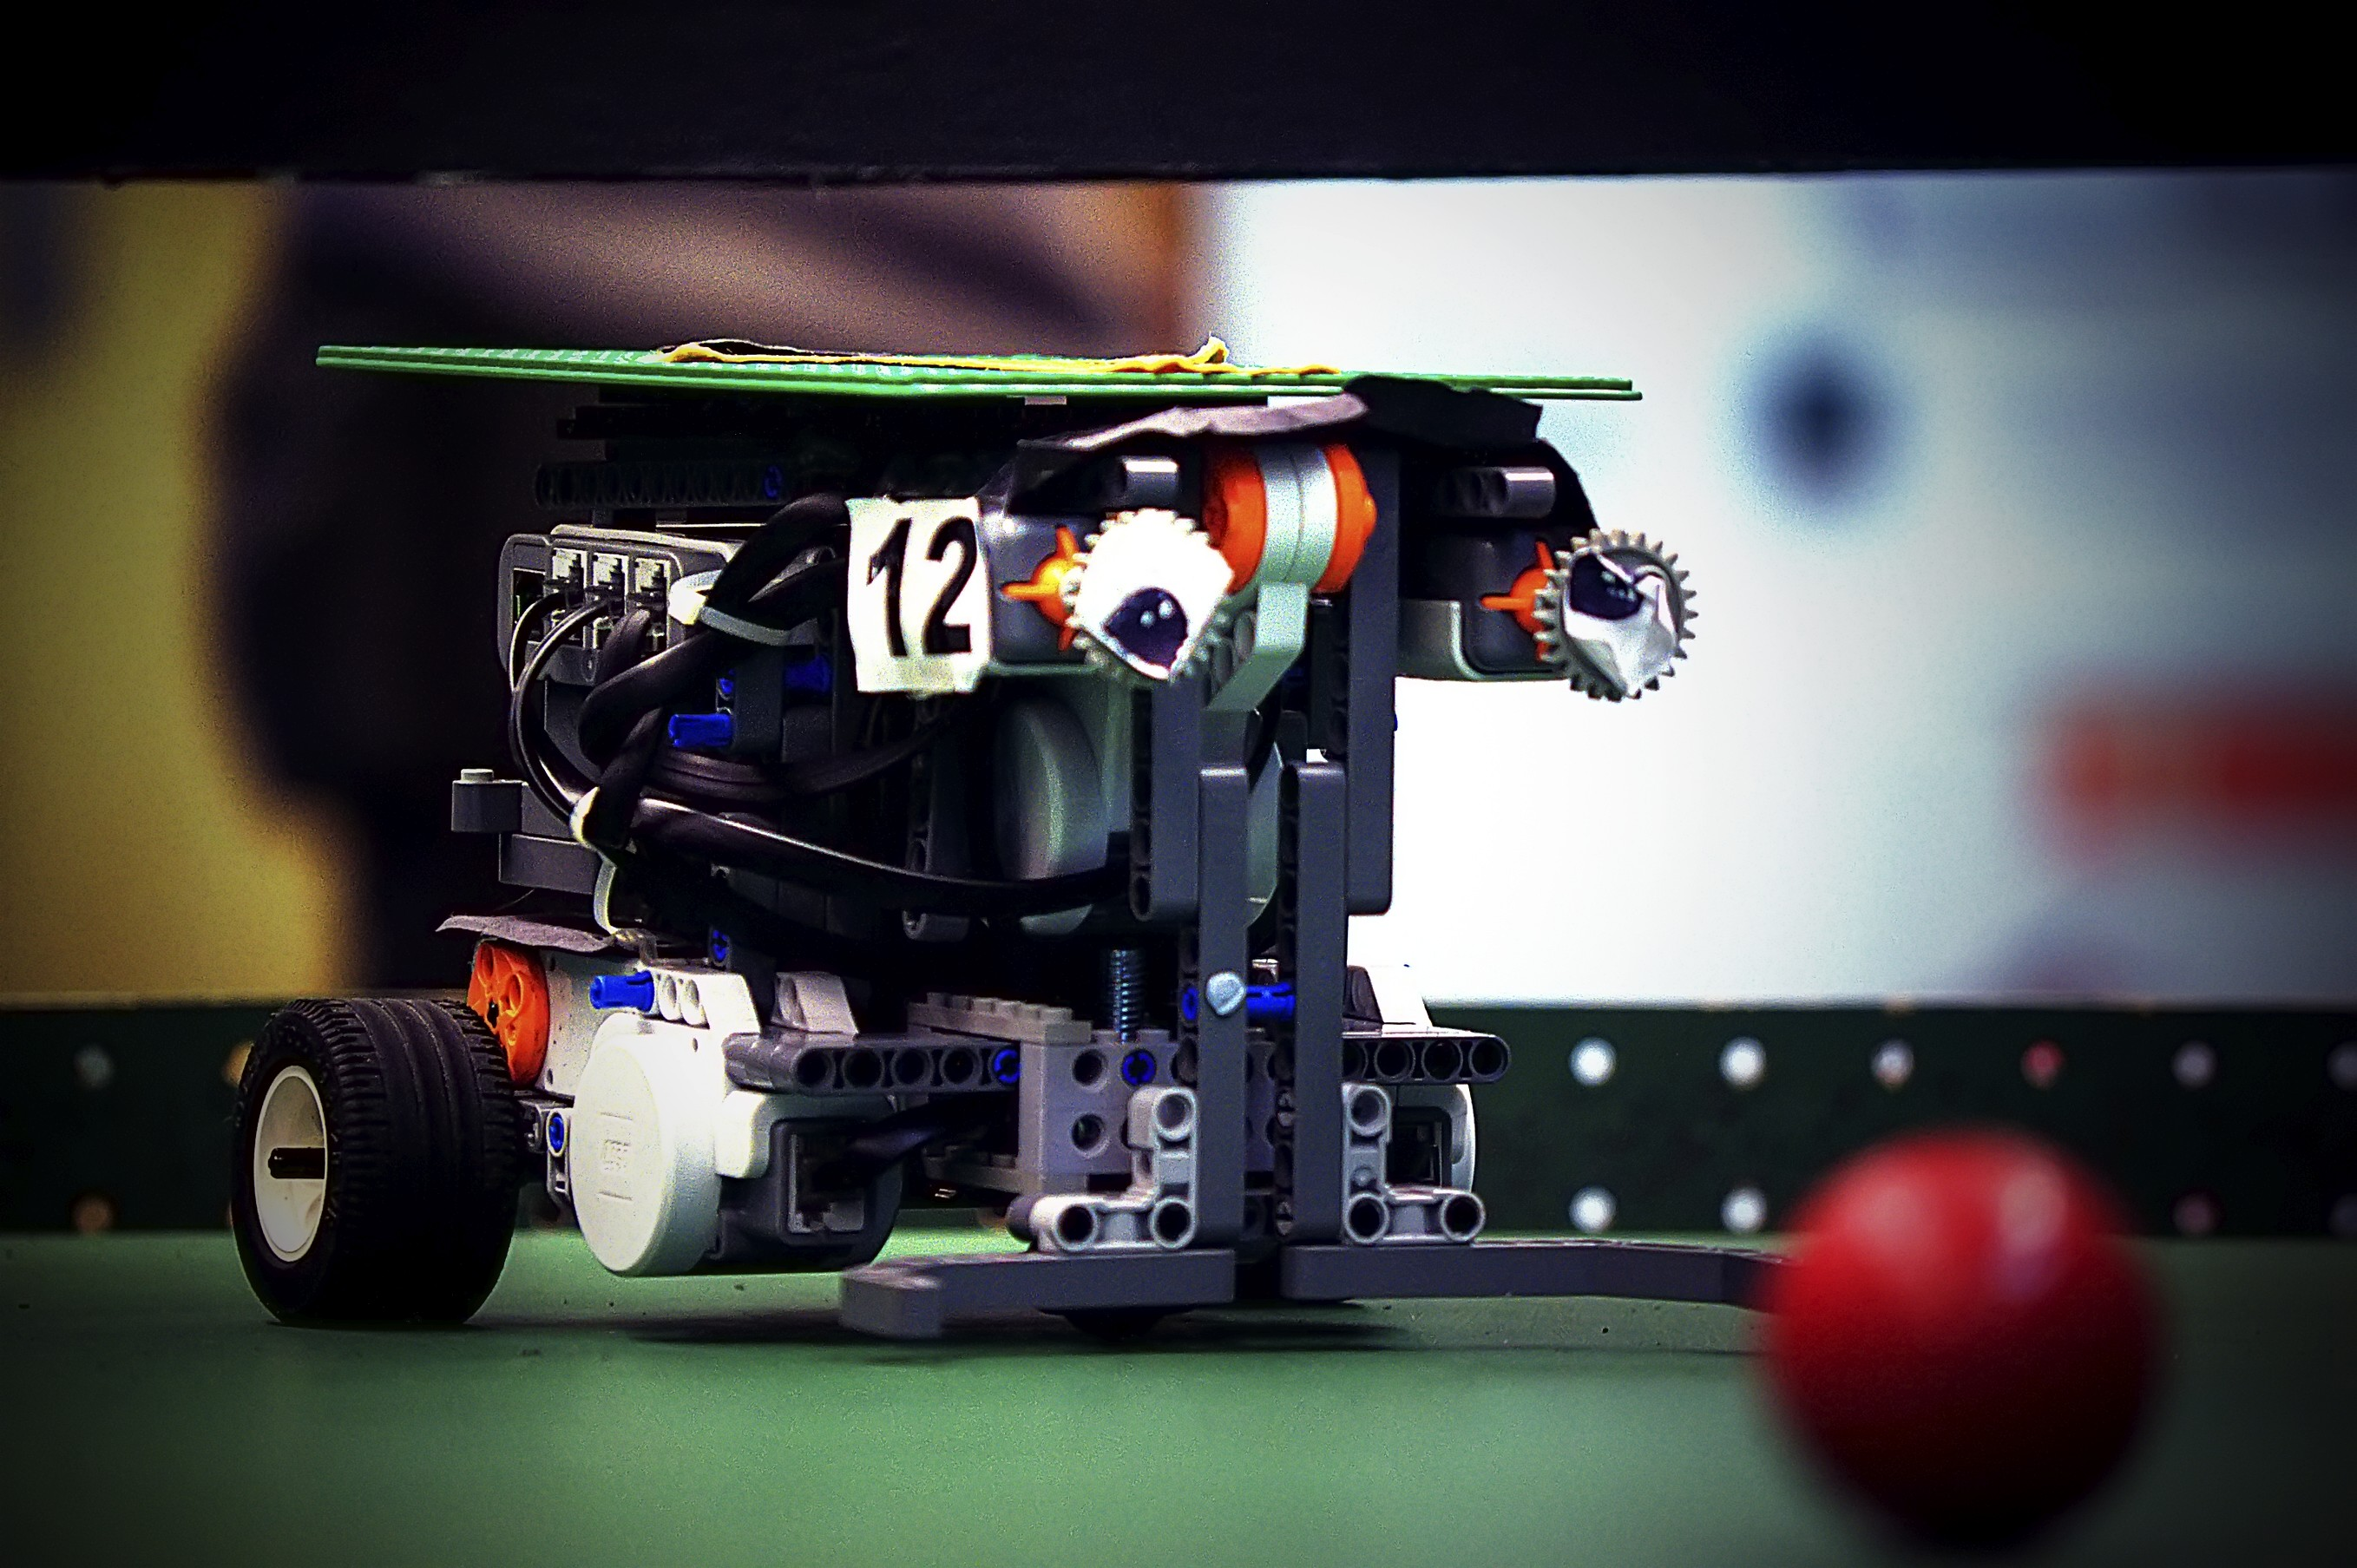
\includegraphics[width=0.25\textwidth] {robotimage.jpg}
\end{center}
\caption{Robot}
\label{fig:agent}
\end{figure} 